\section{Methodology}
\label{sec:methodology}
The methodology adopted relies both, as cited, on a CFD and on a ML part. The CFD part is used to generate the data and test the model while the ML part is used to train the models, both Clustering and NN.

\subsection{CFD dataset}

A CFD simulation campaign is performed to generate the data for the ML part.
Simulations are performed via OpenFOAM-v22.12, an open-source CFD software including an in-house implementation of Actuator Line Model (ALM)\cite{10.1115/1.1471361} based on the open-source library \textit{turbinesFoam}\cite{turbinesFoam}. Both RANS and LES simulations are performed, assuming incompressible flow conditions.
$\vec{U}$ and $p$ fields are solved with the PIMPLE algorithm.
In all the simulations the timestep, corresponding to $2^\circ$ of rotation of the WT rotor, is set to ensure a maximum Courant number of 0.6 with a mean value of 0.02-0.03, while the time integration relied on a first-order Euler scheme. Second order central differences were used for the spatial discretisation of the convective and diffusive terms.

The RANS simulations are performed with the $k$-$\omega$ SST turbulence model \cite{doi:10.2514/3.12149} while the LES simulations are performed with the WALE turbulence model \cite{WALE}.

The following boundary conditions were applied in the RANS case: at the inlet a logarithmic velocity profile was imposed. At the outlet, a zero-gradient condition was set
for the $\vec{U}$ field. No-slip boundary conditions were set for the ground, while freestream conditions were applied to the other lateral boundaries. For pressure a zero-gradient condition was set for all the boundaries.

In the LES case, the same boundary conditions were applied except for the inlet $\vec{U}$ field, where turbulent fluctuations, derived from the Kaimal spectrum, were superimposed to the logarithmic velocity profile. Synthetic inflow conditions based on a spectra-stochastic method are imposed at the inlet derived from the Kaimal power spectral density function \cite{kaimal} following the approach described in \cite{Davidson2007UsingIS}. As done in \cite{Carloni2026}, the turbulent fluctuations are generated by a coded boundary condition, imposing a total of 400 Fourier modes. Continuity is ensured by constraining the orthogonality of the wave numbers and $\vec{U}$. Spatial coherence is imposed through an exponential decay function $\exp(\frac{-\Delta t}{T})$ where $\Delta t$ is the time step of the simulations and $T$ is the time scale of the turbulence considered.

Moreover, to generate the data for the ML regression, a dedicated RANS run was set up by importing the time-averaged $\vec{U}$ and $p$ fields from the LES. Keeping these mean fields frozen, a single iteration of the turbulence-correction loop was then performed, so that the eddy-viscosity field is solved consistently with the imposed LES mean fields, yielding the modified eddy viscosity field $\nu_{t,mod}$. This frozen-field procedure returns, on the RANS grid and within the RANS solver, the eddy-viscosity distribution that the baseline closure would require in order to be consistent with the LES mean flow, and provides the reference against which the data-driven correction is later assessed.

All the model training and testing is performed on the same computational domain, which is a rectangular box where the rotor is placed at 5D from the inlet and 15D from the outlet and $90 m$ from terrain. In spanwise direction the domain extends for 5D on each side of the rotor and in normal direction 8D from the ground.
The domain is obtained by using the \textit{blockMesh} and \textit{snappyHexMesh} utilities of OpenFOAM, with different refinement levels in different regions of the domain to proper solve the turbulent structures in the near wake of the rotor.
Moreover, an inflation layer is applied near terrain. The final mesh consists of around $\sim30.8$ million cells with a minimum cell size of 1.75 m near the rotor and a maximum cell size of 28 m at the domain boundaries while reaching $\sim0.33$ m in the first level of the inflation layer near the ground.
In Fig.~\ref{fig:mesh} the computational domain and the mesh refinement are shown.
\begin{figure*}[h]
    \centering
    \begin{subfigure}[b]{0.49\textwidth}
        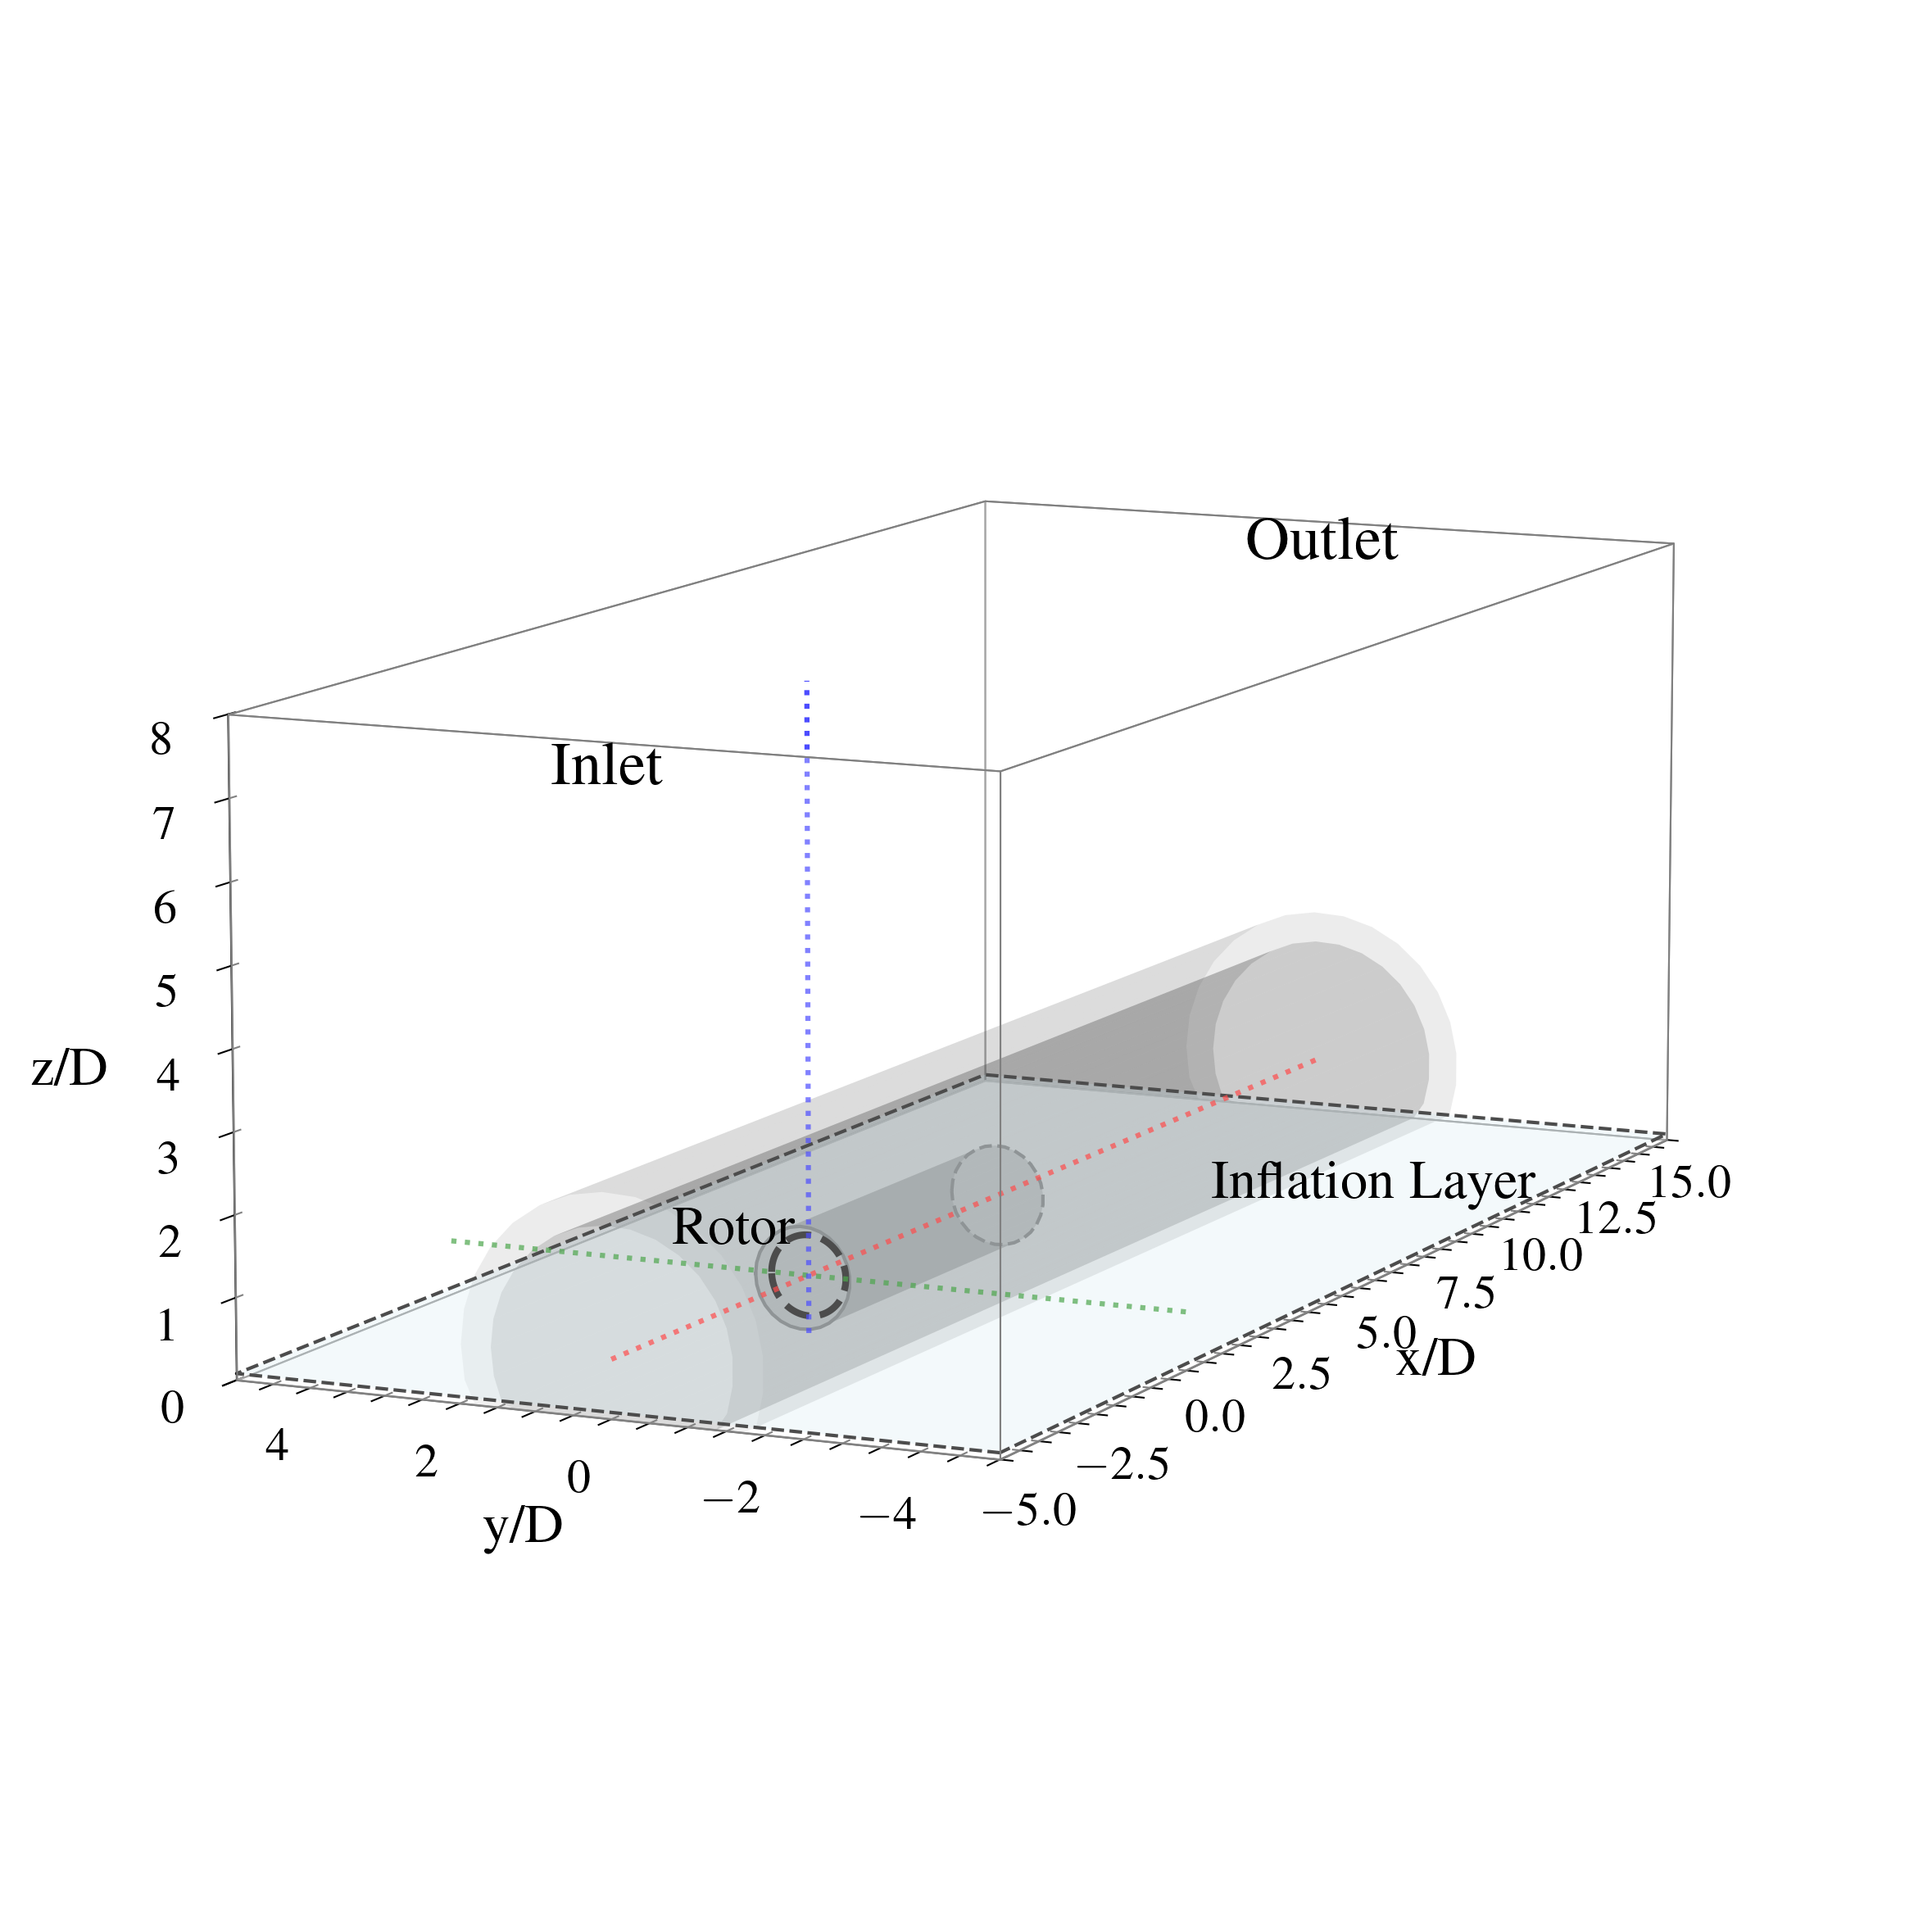
\includegraphics[width=\linewidth, trim= 0 100 0 0,clip]{methodology/img/domain_3d_abl.png}
        \caption{}
    \end{subfigure}
    \hfill
    \begin{subfigure}[b]{0.49\textwidth}
        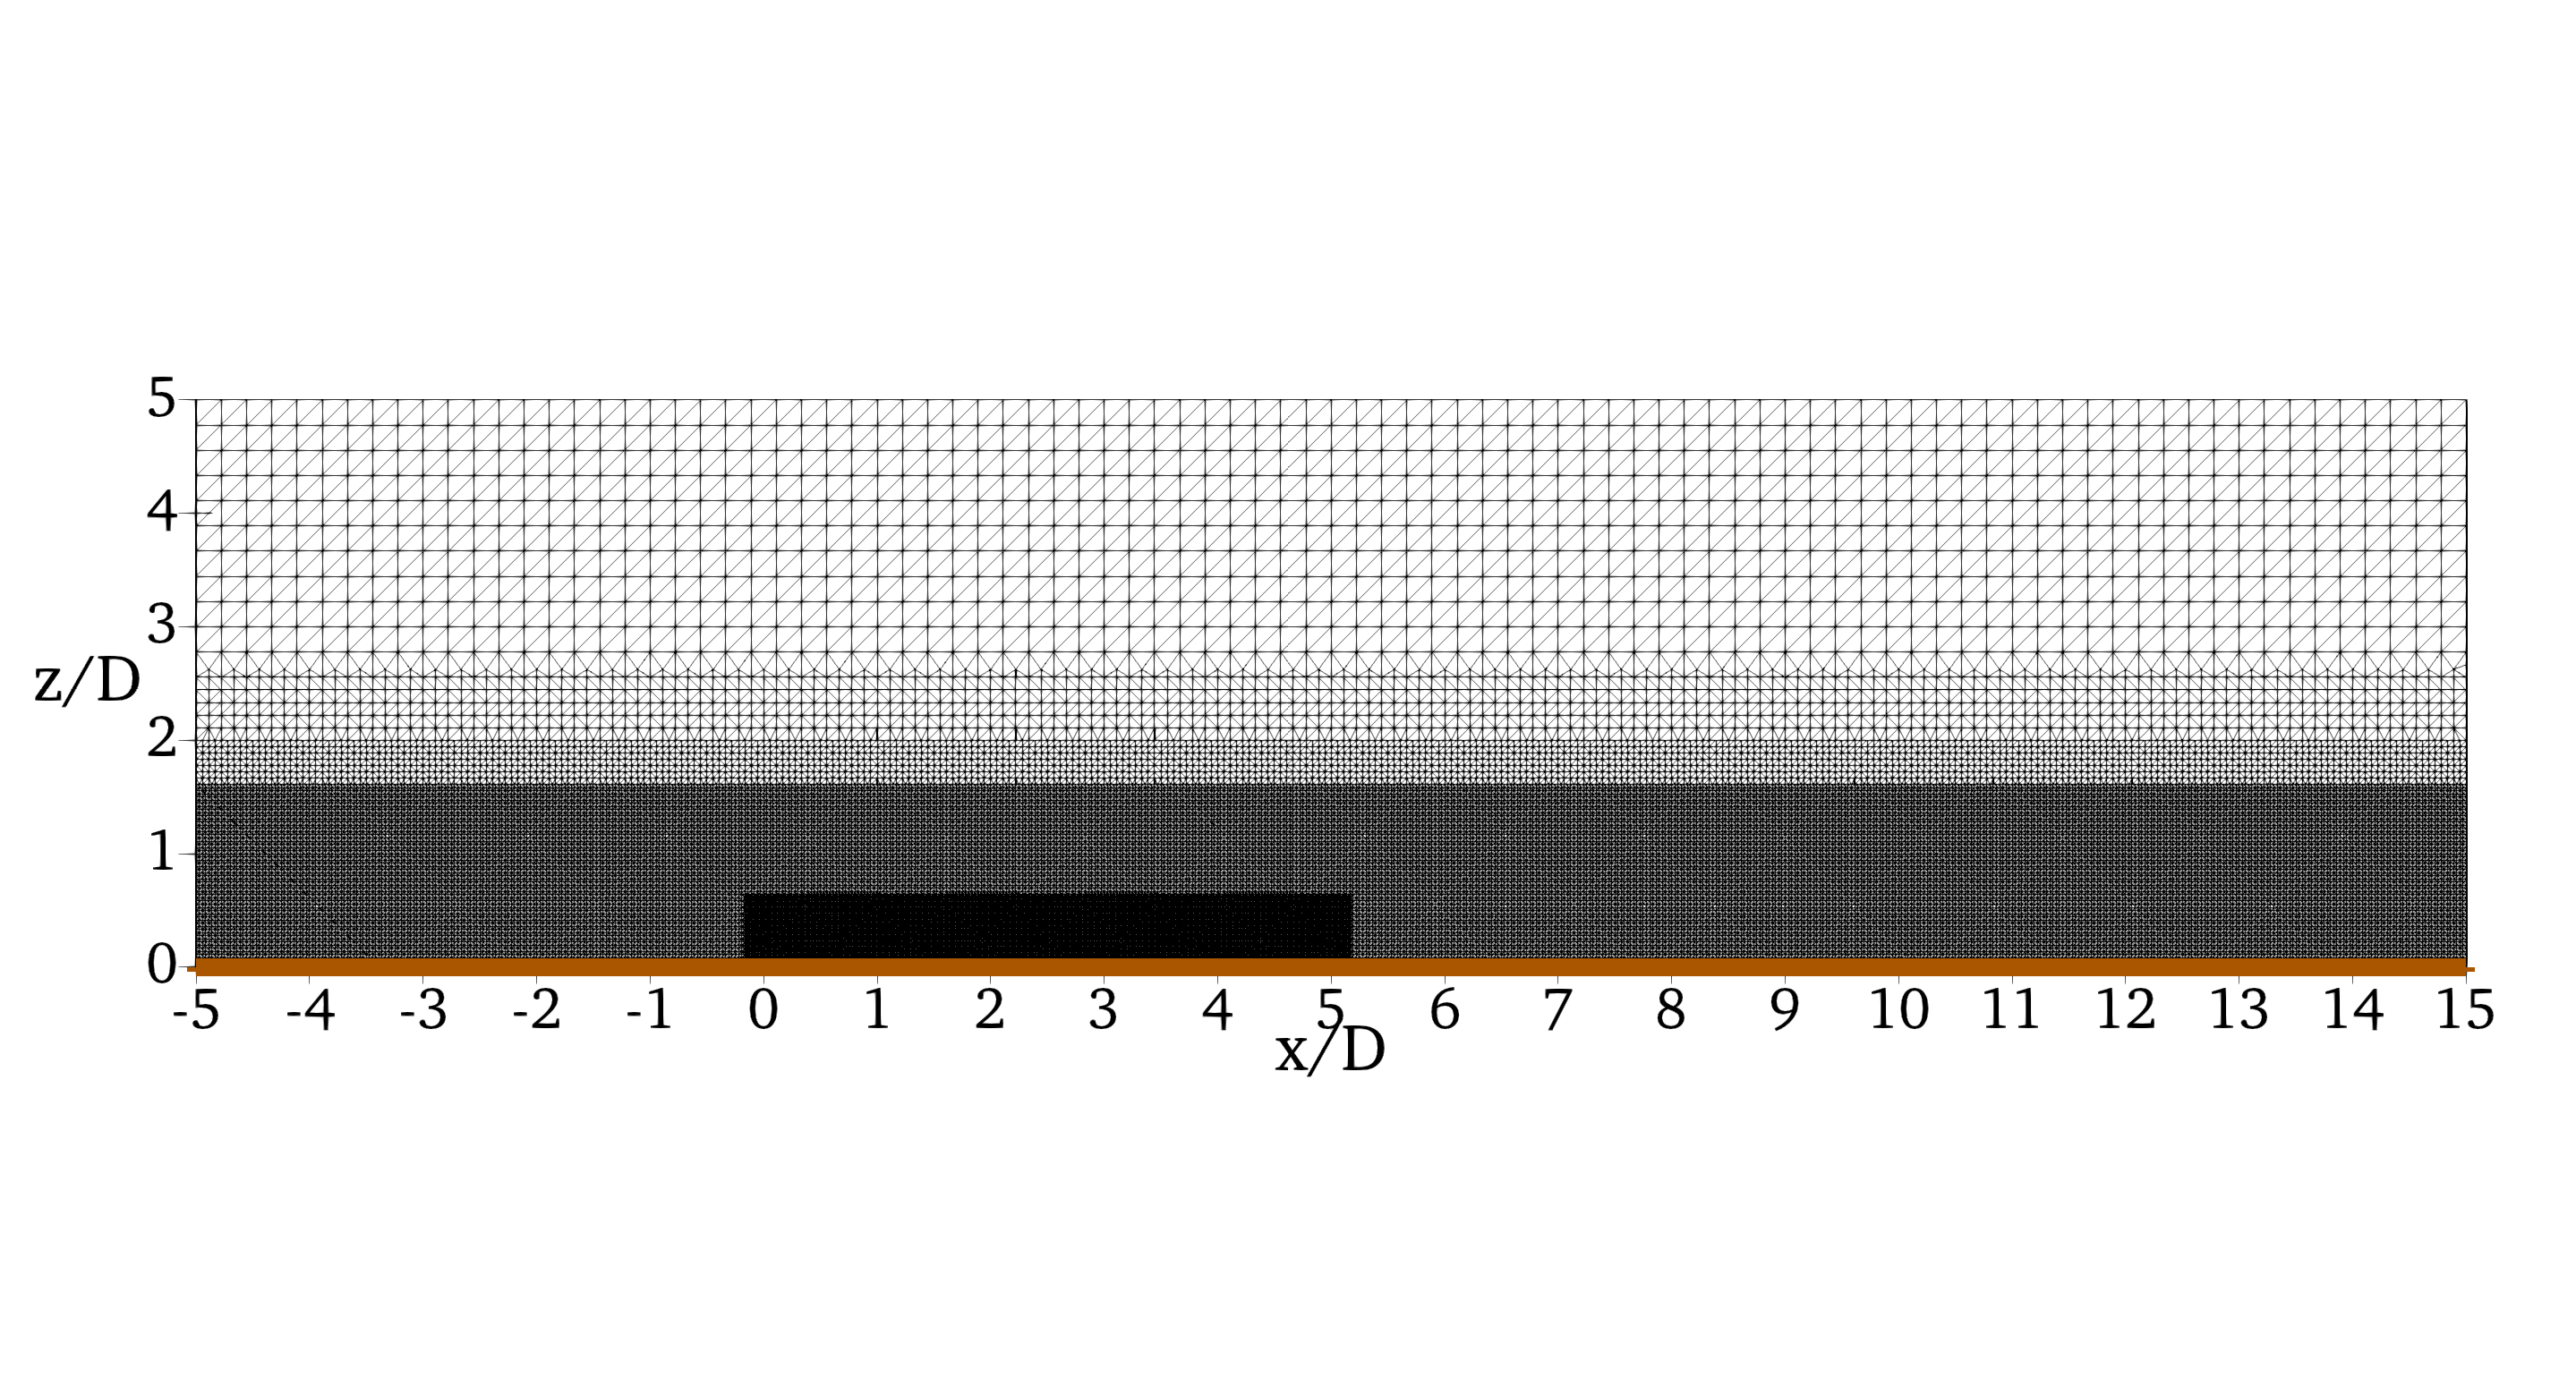
\includegraphics[width=\linewidth]{methodology/img/slice_mesh.png}
        \caption{}
    \end{subfigure}
    \caption{Computational domain (a) and refinement levels represented in (b).}
    \label{fig:mesh}
\end{figure*}

Moreover, the same domain has been used to test the trained models and the mesh refinement influence on the results: while the computational domain and the refinement levels are the same, the minimum and maximum cell size are varied to generate coarser meshes, leading to $\sim15.9$, $\sim9.1$ and $\sim4.2$ million cells with a minimum cell size of $\sim2.25$ m, $\sim2.82$ m and $\sim3.94$ m respectively near the rotor and a $\times 16$ cell size at the domain boundaries.

The CFD simulations were run on a high-performance computing workstation equipped with two AMD EPYC 9534 64-Core processors, for a total of 128 physical cores and 256 threads.

The three types of simulations (RANS, LES and modified RANS) results are shown in Fig.~\ref{fig:cfds}.
\begin{figure*}[h]
    \centering
    \begin{subfigure}[b]{0.32\textwidth}
        \centering
        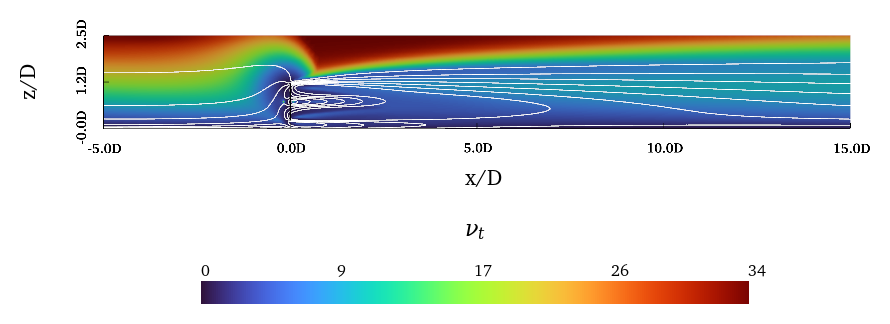
\includegraphics[width=\linewidth]{methodology/img/cfds_rans_nut_xz.png}
        \caption{}
    \end{subfigure}
    \hfill
    \begin{subfigure}[b]{0.32\textwidth}
        \centering
        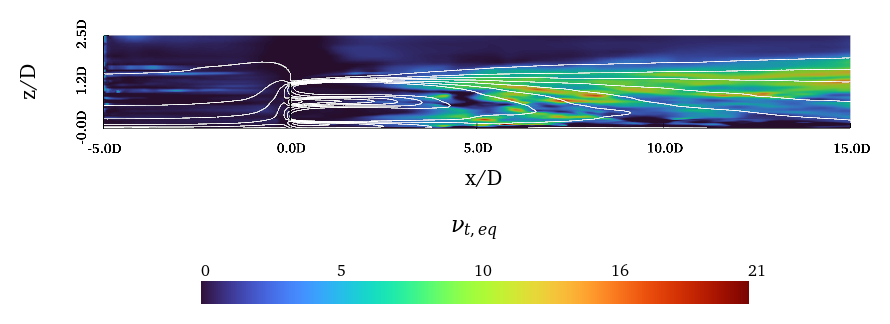
\includegraphics[width=\linewidth]{methodology/img/cfds_les_nutEq_xz.png}
        \caption{}
    \end{subfigure}
    \hfill
    \begin{subfigure}[b]{0.32\textwidth}
        \centering
        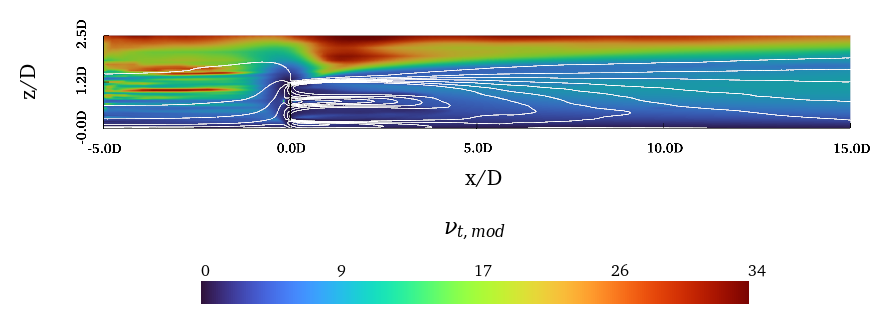
\includegraphics[width=\linewidth]{methodology/img/cfds_modified_nut_xz.png}
        \caption{}
    \end{subfigure}
    \caption{Eddy viscosity fields on the $xz$ plane: (a) original RANS $\nu_t$, (b) LES-equivalent $\nu_{t,eq}$, and (c) modified RANS $\nu_{t,mod}$. The black and white isolines highlight the velocity magnitude contours for RANS simulation and mean velocity ones for the LES and modified RANS simulations.}
    \label{fig:cfds}
\end{figure*}


\subsection{ML methodologies}
\label{sec:ML_part}
Different ML techniques are employed in this study to predict the modified eddy viscosity field $\nu_t$ and the corresponding $\vec{U}$, $p$ and $k$ fields. These methods include both CA and NN, as described in the following.

All the ML models were trained on the same workstation, equipped with an Intel Core i9-10980XE CPU running at 3.00 GHz, with 18 physical cores and 36 threads, and a single NVIDIA Quadro RTX 6000 GPU with 24 GB of dedicated memory.

\subsubsection{Clustering model}
\label{sec:clustering}
This work entails the use of a CA as a cornerstone of all the analysis. This, as in \cite{Carloni2026,Clustering_tieghi}, is done to identify the different flow regions in the wake of the rotor, which are characterised by different dynamics and thus require different modeling approaches.
Moreover, the usage of the CA has an advantage in terms of interpretability of the results and in terms of generalisation capabilities of the trained models: in fact it allows to move from a cell-wise prediction of the $\nu_t$ field to a region-wise prediction, which is more robust and less affected by the mesh refinement and by the geometrical details of the domain.

In fact, clustering algorithms are unsupervised ML techniques that allow to group data points in clusters based on their similarity.
Many different CAs exist in literature and with different characteristics, but in this work the K-means algorithm is used as in \cite{Carloni2026,Clustering_tieghi} for many reasons: it is proven to be effective in identifying the different flow regions in the wake of the rotor and its computational complexity scales well with the size of the dataset, which is a crucial aspect in this study given the large amount of data generated by the CFD simulations. 
The clustering pipeline was implemented in a Python environment leveraging the \textit{scikit-learn} \cite{scikit-learn} open-source library. The K-means algorithm partitions the dataset by minimising the within-cluster sum of squares, the quantity reported by \textit{scikit-learn} as the \textit{inertia} of the clustering and defined as:
\begin{equation}
    \mathrm{Inertia} = \sum_{i=1}^{K} \sum_{x_j \in C_i} \lVert x_j - \mu_i \rVert^2 ,
\end{equation}
where $K$ is the number of clusters, $C_i$ is the set of data points in cluster $i$, $x_j$ is a data point belonging to cluster $i$ and $\mu_i$ is its centroid. The algorithm iteratively assigns each data point to the nearest centroid and updates the centroids until convergence is reached.
To select the optimal number of clusters, the elbow method is used, analysing the inertia as a function of the number of clusters $K$: the chosen $K$ corresponds to the point beyond which additional clusters yield only a marginal reduction of the inertia.
To ensure a correct clustering of the data, the features are previously normalised via a Min-Max normalisation \cite{scikit-learn},
\begin{equation}
    x' = \frac{x - x_{min}}{x_{max} - x_{min}} .
\end{equation}
Then, as done in \cite{Carloni2026,Clustering_tieghi}, the features are projected on a cylindrical reference system centered on the rotor and a subset of them is selected based on the PCA analysis and on the physical understanding of the problem, to ensure a correct clustering of the data both in terms of data analysis and physical interpretation of the results.
Since the exact pipeline has been already described in previous works \cite{Carloni2026,Clustering_tieghi}, here only the main results are presented (i.e., the optimal number of clusters  and clustering features).
Results of the clustering methodology are reported in Sec.~\ref{sec:clustering_results}.

A brief review of the clustering pipeline together with the CFD one is reported in Fig.~\ref{fig:methodology_pipeline}.
\begin{figure*}[h]
    \centering
    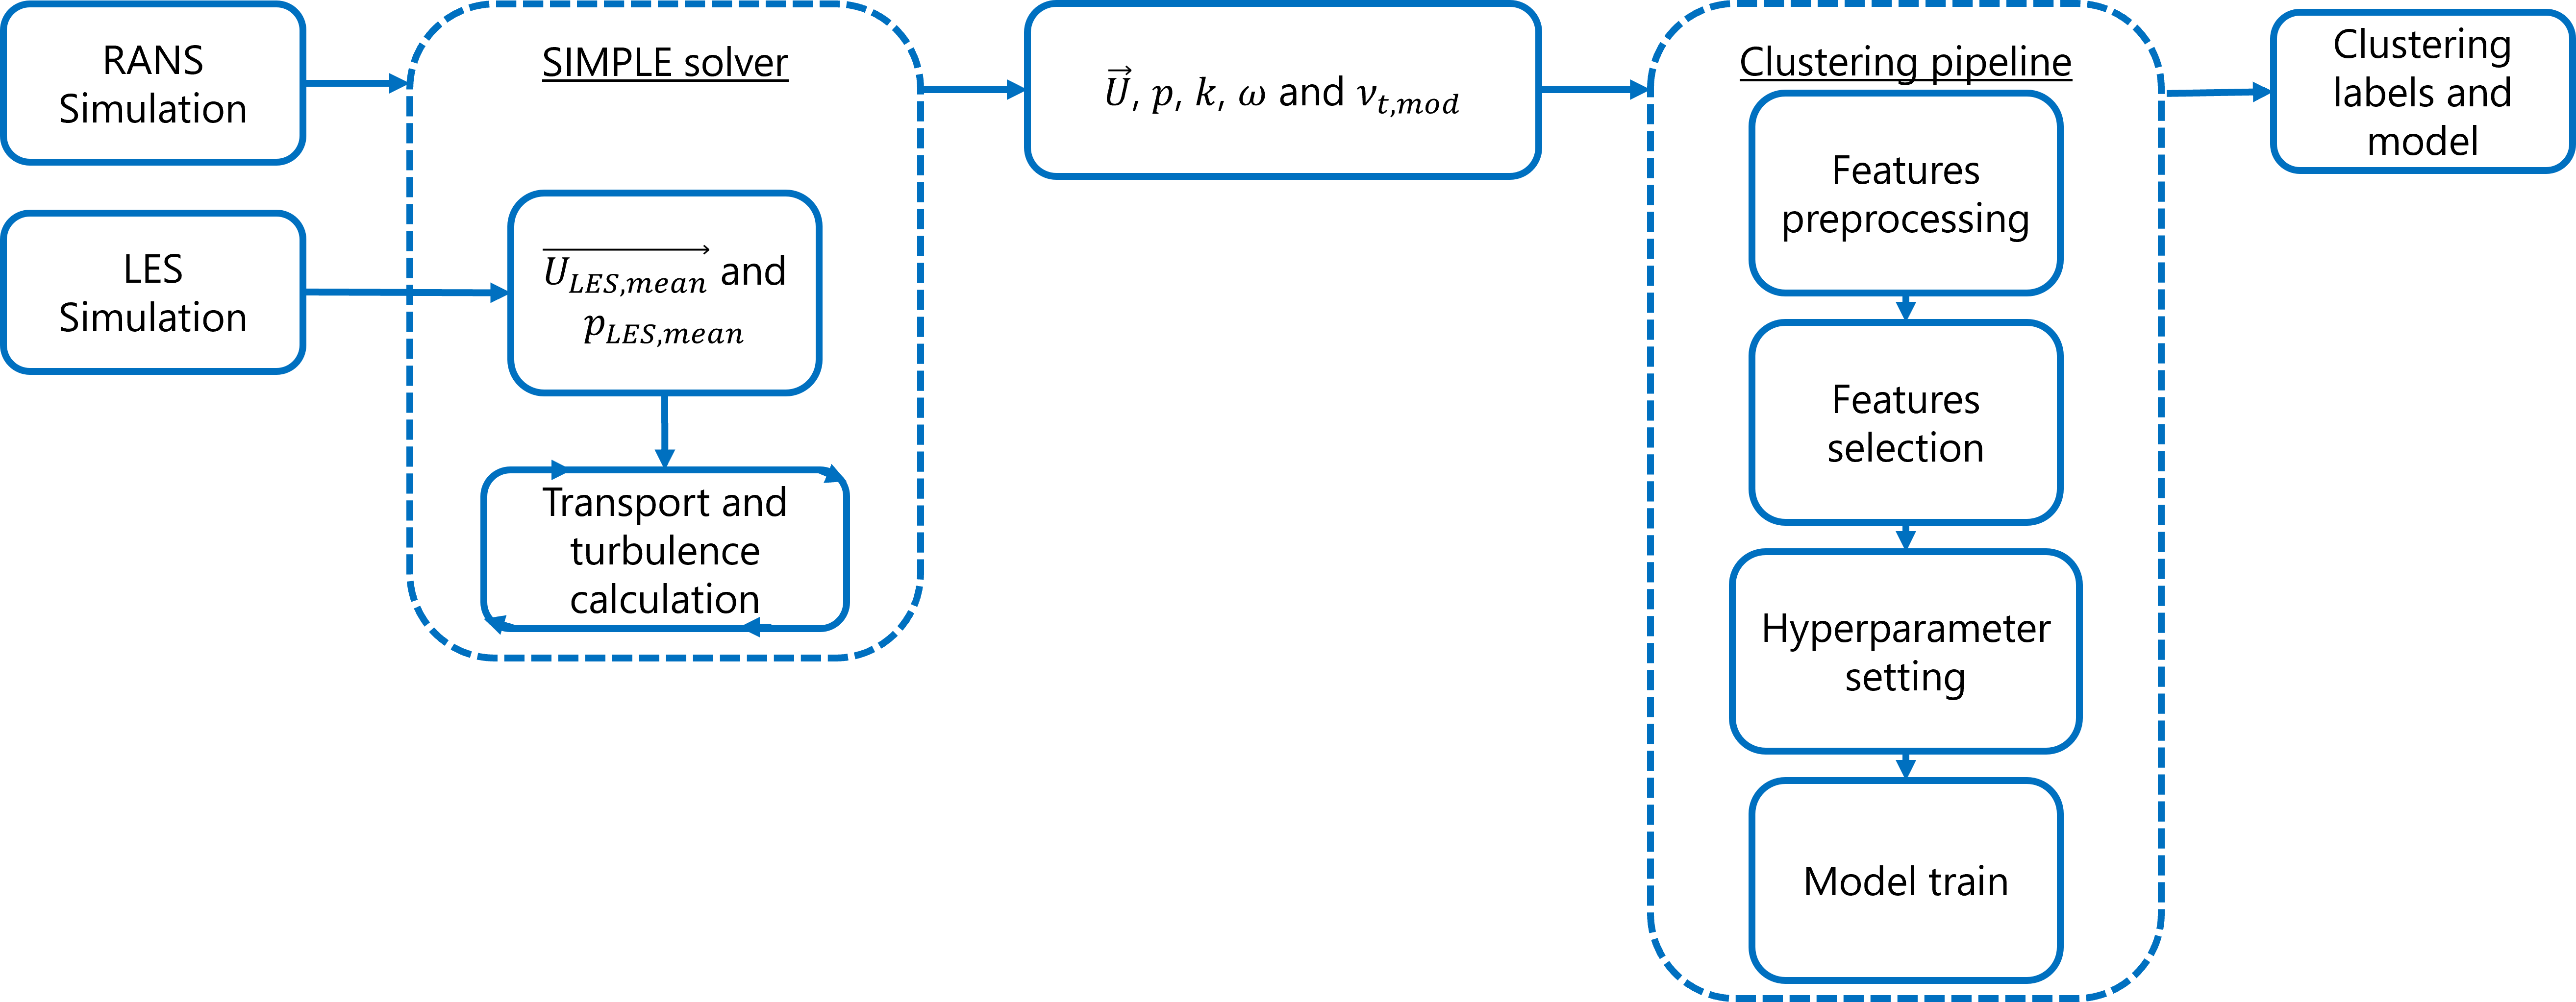
\includegraphics[width=1\textwidth]{methodology/img/clustering_pipelinepng.png}
    \caption{CFD and ML pipeline.}
    \label{fig:methodology_pipeline}
\end{figure*}

\subsubsection{NN model}
\label{sec:NN}
Finally, after the clustering of the data, a NN is trained to predict the $\nu_{t,ML}$ field.
In this work, $\nu_t$ denotes the kinematic turbulent viscosity, namely the scalar field used in the Boussinesq approximation to model the effect of the unresolved turbulent stresses on the mean momentum equation. It enters the RANS equations through the effective viscosity,
\begin{equation}
    \nu_{eff} = \nu + \nu_t ,
\end{equation}
where $\nu$ is the molecular kinematic viscosity of the fluid. The reference quantity used to define the regression target is the correction between the baseline RANS eddy viscosity $\nu_{t,\mathrm{RANS}}$ and an equivalent LES eddy viscosity $\nu_{t,eq}$.

The field $\nu_{t,eq}$ is obtained by projecting the deviatoric part of the LES turbulent stress tensor onto the Boussinesq form. The total deviatoric turbulent stress is written as the sum of the resolved and subgrid-scale contributions,
\begin{equation}
    \Sigma_{ij}^{dev} =
    \left(R_{ij}^{res}\right)^{dev} + \tau_{ij}^{sgs,dev}
    \simeq -2 \nu_{t,eq} S_{ij},
\end{equation}
where $S_{ij}$ is the resolved strain-rate tensor and $R_{ij}^{res}$ is the resolved stress tensor. Assuming a Smagorinsky-type subgrid contribution,
\begin{equation}
    \tau_{ij}^{sgs,dev} = -2 \nu_{sgs} S_{ij},
\end{equation}
$\nu_{t,eq}$ is evaluated as the scalar viscosity that minimises the Frobenius norm
\begin{equation}
    J(\nu_t) =
    \left[
    \left(R_{ij}^{res}\right)^{dev}
    -2\nu_{sgs}S_{ij}
    +2\nu_t S_{ij}
    \right]
    :
    \left[
    \left(R_{ij}^{res}\right)^{dev}
    -2\nu_{sgs}S_{ij}
    +2\nu_t S_{ij}
    \right].
\end{equation}
The optimality condition $\partial J/\partial \nu_t=0$ gives
\begin{equation}
    \nu_{t,eq}
    =
    \nu_{sgs}
    -
    \frac{\left(R_{ij}^{res}\right)^{dev}S_{ij}}
    {2S_{ij}S_{ij}} .
\end{equation}
By construction, $\nu_{t,eq}$ is the scalar eddy viscosity that best reproduces, in a least-squares sense, the deviatoric LES turbulent stress within the Boussinesq framework. It therefore does not encode the full Reynolds-stress anisotropy; this is a deliberate choice, consistent with the scalar closure targeted here and with the requirement that the resulting field be directly usable by a standard eddy-viscosity solver, where the goal is to reproduce the LES turbulent mixing rather than its tensorial structure.

Rather than predicting $\nu_{t,eq}$ directly, the NN is trained to predict the discrepancy between the RANS eddy viscosity and the LES-equivalent eddy viscosity,
\begin{equation}
    \Delta \nu_t = \nu_{t,eq} - \nu_{t,\mathrm{RANS}}.
\end{equation}
The final data-driven eddy viscosity is therefore reconstructed as
\begin{equation}
    \nu_{t,ML} = \nu_{t,\mathrm{RANS}} + \Delta \nu_{t,ML}.
\end{equation}
This formulation allows the network to learn the correction required to move from the baseline RANS eddy viscosity to the LES-equivalent eddy viscosity used as target closure.

The regression model is a Multi-Layer Perceptron (MLP), implemented in TensorFlow-Keras \cite{tensorflow2015-whitepaper}, with a single scalar output corresponding to $\Delta \nu_{t,ML}$. The input vector is defined at cell level and includes $\vec{U}_{cyl}$, $k$, $\nu_{t,\mathrm{RANS}}$, the distance from the assigned cluster centroid in the normalised clustering space, the non-dimensional vertical and axial coordinates $z/D$ and $x/D$, and the cluster labels. The continuous features are standardised using a Standard Scaler, while the cluster labels are encoded through one-hot encoding. The target $\Delta \nu_t$ is also standardised before training.

Prior to the split, cells in the far-upstream inflow region ($x/D < -2.5$) are excluded from the training and validation sets, as the NN performance in that zone is inherently limited by the synthetic inlet boundary condition; this reduces the dataset from $\sim 180k$ cells to $\sim 160k$ cells retained for training and validation. The remaining points are split into training and validation subsets using an 80/20 split, stratified with respect to the cluster labels in order to preserve the same distribution of flow regions in both sets. During training, sample weights are introduced to compensate for cluster imbalance through inverse-frequency weighting. An additional axial weight is applied to increase the relevance of downstream wake samples, according to
\begin{equation}
    w_{ax} = 1 + \max(x/D,0),
\end{equation}
and the final sample weight is obtained as the product of the cluster and axial weights.

The MLP architecture is composed of a sequence of fully connected residual blocks. Each block contains a Dense layer with L2 kernel regularization, Layer Normalization, a GELU activation function and Dropout. When residual connections are enabled, the block input is added to the block output; if the two tensors have different dimensions, the shortcut is first projected through a linear Dense layer. The hidden-layer widths are progressively reduced according to
\begin{equation}
    n_i = \max \left( \mathrm{round}(n_0 r^{i-1}), 32 \right),
\end{equation}
where $n_0$ is the initial number of neurons and $r$ is a width-decay factor. This is done in order to reduce the complexity of the model and prevent overfitting and also to catch more complex relationships between the input features in the first layers and to produce a more compact representation. The output layer is a linear Dense layer with one neuron. The model is trained by minimising a weighted Huber loss using the Adam optimizer, while the mean absolute error is monitored as an additional metric.

The architecture and training hyperparameters are fixed through a manual preset, selected from preliminary tests and kept unchanged for the reported training. The adopted configuration is reported in Tab.~\ref{tab:nn_manual_configuration}.

\begin{table}[h]
    \centering
    \caption{Manual configuration adopted for the MLP training.}
    \label{tab:nn_manual_configuration}
    \begin{tabular}{lc}
        \hline
        Hyperparameter & Value \\
        \hline
        Hidden blocks & 7 \\
        Initial neurons $n_0$ & 192 \\
        Width decay $r$ & 0.78 \\
        Hidden-layer widths & 192, 150, 117, 91, 71, 55, 43 \\
        Activation function & GELU \\
        Layer Normalization & True \\
        Residual connections & True \\
        Dropout rate & 0.05 \\
        L2 regularization & $1\cdot10^{-4}$ \\
        Learning rate & $1.5\cdot10^{-4}$ \\
        Huber $\delta$ & 1.0 \\
        Batch size & 128 \\
        \hline
    \end{tabular}
\end{table}

The final model is trained with early stopping on the validation loss and a learning-rate reduction on plateau. The maximum number of epochs is controlled by the training configuration and was set to 400 in the reported run. In addition to the training and validation loss, the RMSE and physical-space validation metrics are monitored during training.

Results of the NN training and testing are reported in Sec.~\ref{sec:NN_results} as for the clustering ones.
MLP training pipeline is summarised in Fig.~\ref{fig:mlp_pipeline}.
\begin{figure*}[h]
    \centering
    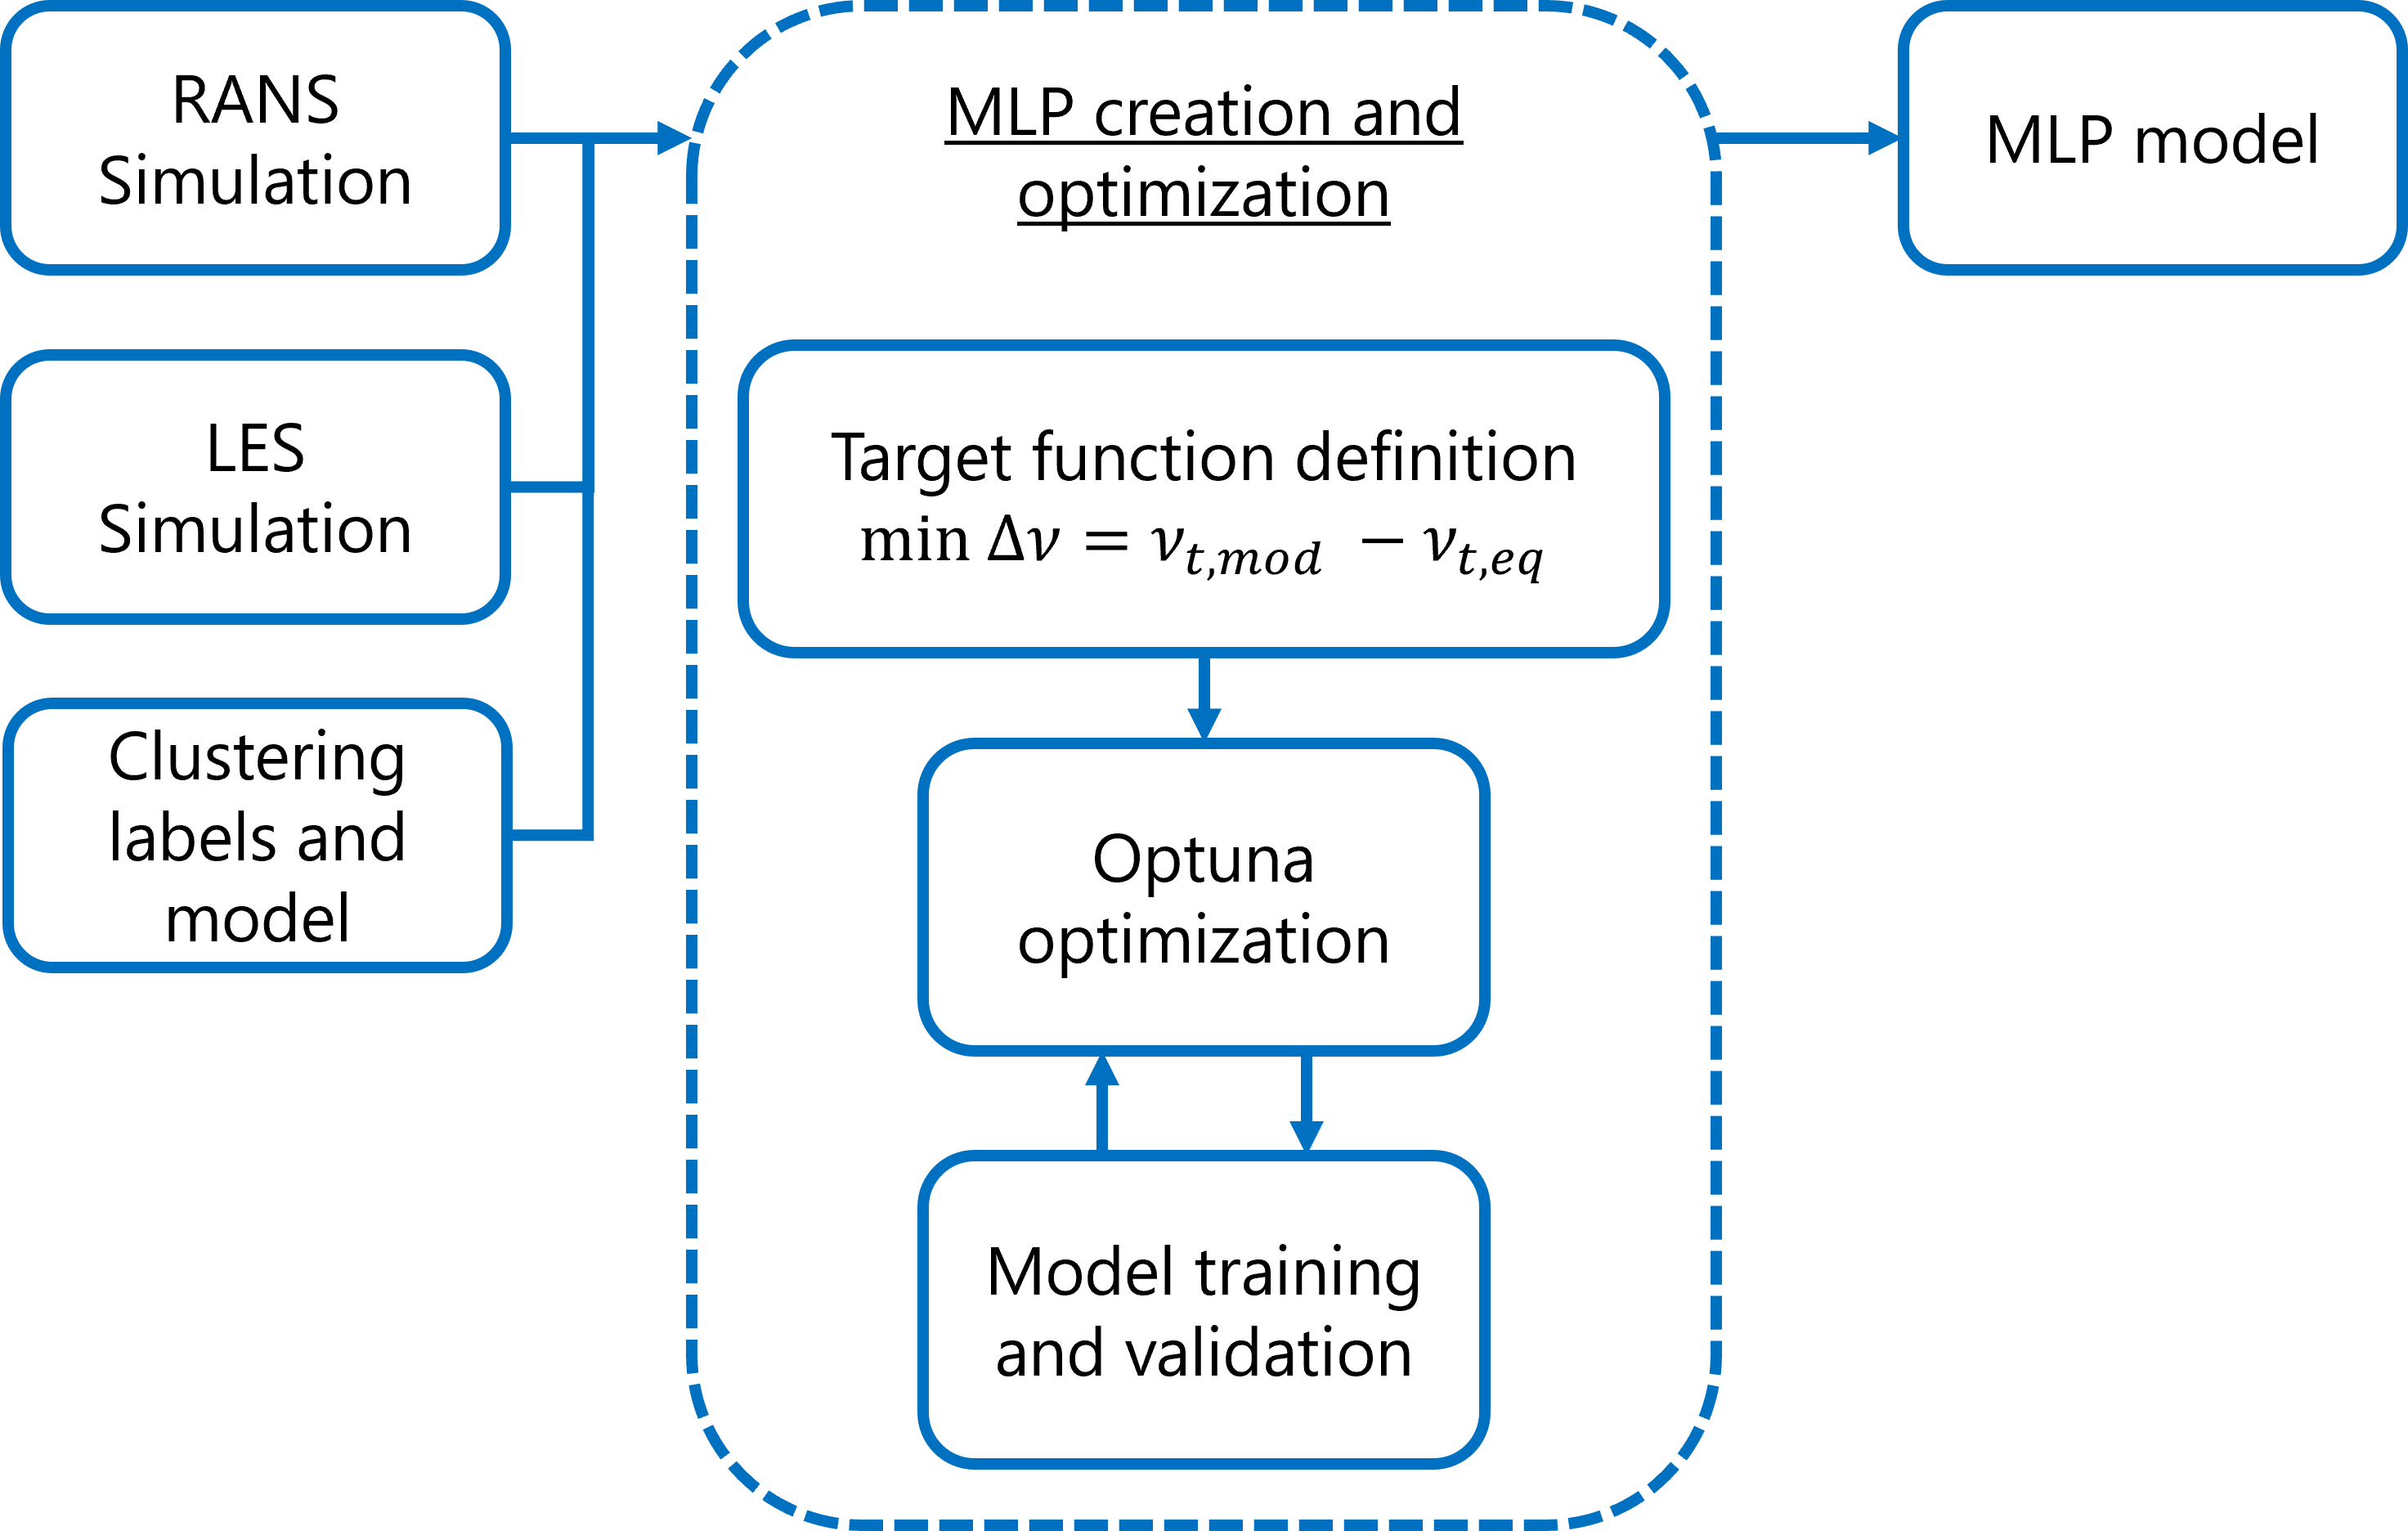
\includegraphics[width=0.6\textwidth]{methodology/img/NNpipeline.png}
    \caption{MLP training pipeline.}
    \label{fig:mlp_pipeline}
\end{figure*}

\subsection{ML-based RANS model implementation}
\label{sec:ml_pimple_pipeline}
Finally all the trained models are implemented in the RANS solver of OpenFOAM to test their performance in a predictive setting. To do so, a modified version of the PIMPLE algorithm is implemented as in Fig.~\ref{fig:pimple_pipeline}.
\begin{figure*}
    \centering
    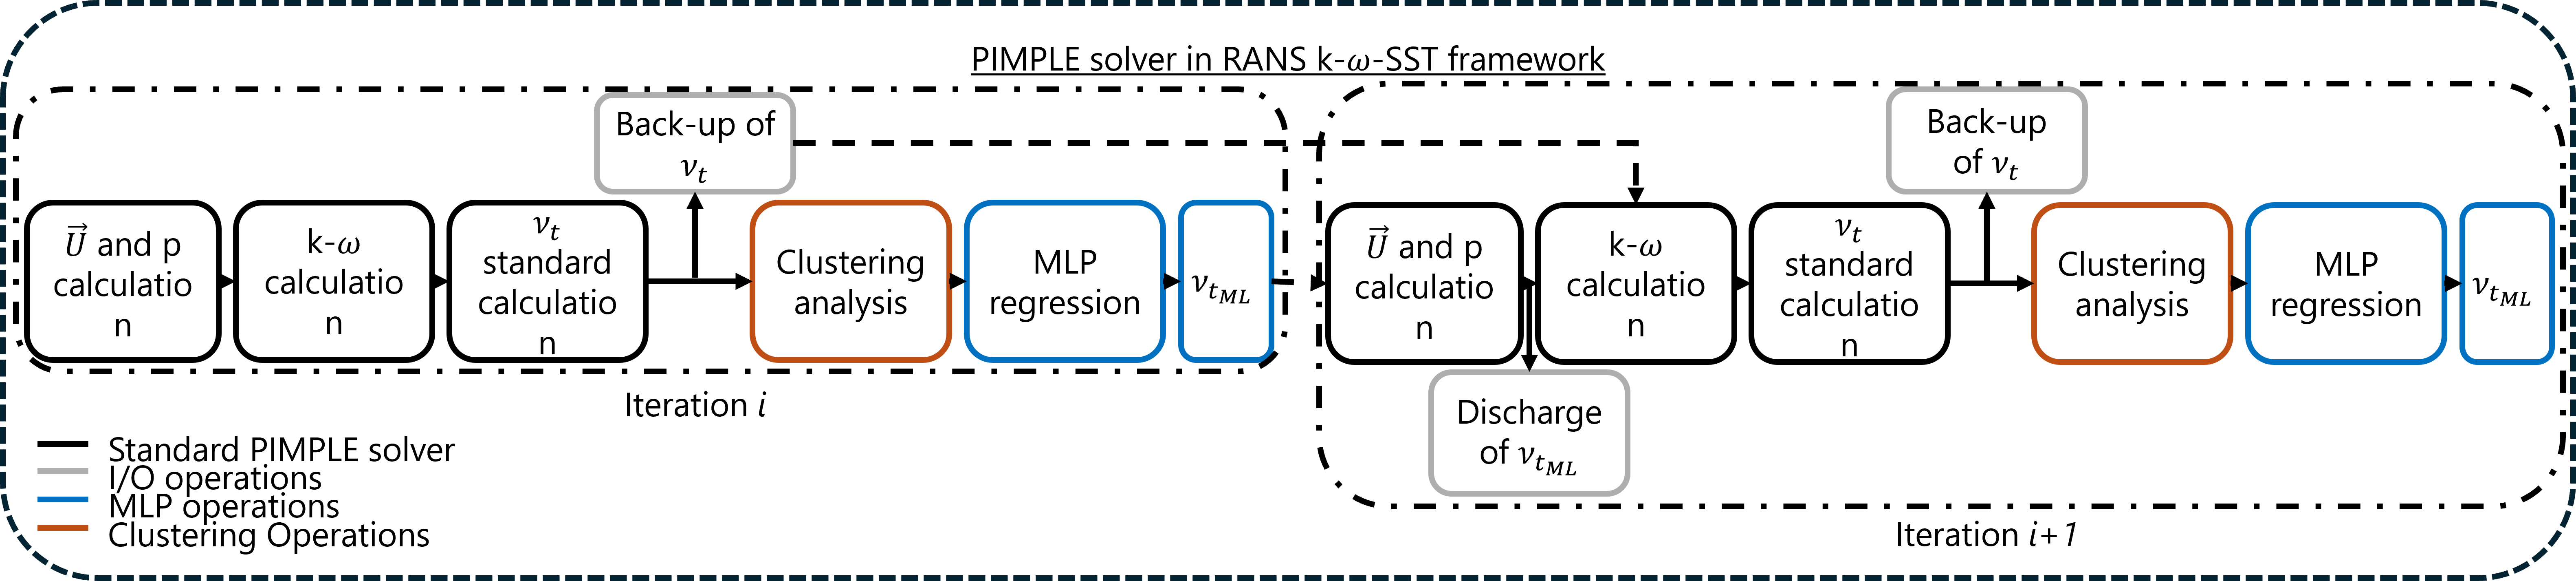
\includegraphics[width=1\textwidth]{methodology/img/solver_pipeline.png}
    \caption{ML-based PIMPLE algorithm.}
    \label{fig:pimple_pipeline}
\end{figure*}
The $\vec{U}_{cyl}$-$p$ PIMPLE internal loop is not modified, while the turbulence correction loop is: the first iteration of the solver is executed with the standard $k$-$\omega$ SST model to compute the $\vec{U}$, $p$, $k$, $\omega$ and $\nu_t$ fields, then the clustering model is applied to assign a cluster label to each cell and the NN is applied to predict the $\nu_{t,ML}$ field; this is then used, in the second iteration of the solver, to compute the $\vec{U}$ and $p$ fields, while the $k$ and $\omega$ fields are still computed with the standard SST model stored in the first iteration and then corrected again with the NN; the same procedure is repeated for the following iterations of the solver.

By design, only the eddy viscosity entering the momentum equations is replaced by the data-driven field, whereas the $k$ and $\omega$ transport equations retain the standard SST formulation and its boundedness treatment. This keeps the correction confined to the closure term and preserves the numerical robustness of the baseline solver: across all the grids and inflow velocities tested, the modified solver reached a stable statistically-steady state without any ad hoc relaxation or limiter on the predicted field. It is also worth stressing that the clustering and NN inference are the only components added to the solver loop, so that the data-driven model is fully embedded in the CFD solver and used predictively, with no LES information supplied at run time.
